\section{Consistency in distributed systems}
\label{sec:distrsys}

A distributed system, broadly construed, is a collection of
independent entities that cooperate to solve a problem that cannot be
individually solved \cite{kshemkalyani_singhal_2008}. Here we are
concerned with the sorts of distributed systems involved in civil
aviation in the context of disaster response scenarios like combating
wildfires and providing hurricane relief. In these scenarios, entities
like emergency responders, firefighters, crewed and uncrewed aircraft
teams, air traffic controllers, and other personnel cooperate to solve
shared tasks like navigating safely, delivering resources,
extinguishing fires, and collecting and sharing data. A paramount
concern in all of our use cases is that the system must ensure strong
safety guarantees.

Safely coordinating the actions of distributed agents is a challenge
for distributed computing. Singhal and Shivaratri
\cite{10.5555/562065} characterized a distributed computing system as
\begin{quotation}
  A collection of computers that do not share common memory or a
  common physical clock, that communicate by message passing over a
  communication network, and where each computer has its own memory
  and runs its own operating system.
\end{quotation}
``Computers" here should be understood broadly, taken to include
aircraft systems like ADS-B, portable communications equipment,
satellites, vehicle-mounted personal computers, or smartphones carried
by firefighters in the field.

Absence of a common memory implies that all communication between
system nodes takes place over the network, rather than by writing data
to mutually accessible memory. In general, and particularly during
disaster response scenarios, message delivery is neither guaranteed
nor instantaneous. For example, two firefighting ground teams may not
be able to communicate with each other over a radio network if the
teams are separated by a tall ridgeline. Handling these sorts of
challenges gracefully---for example, automatically redirecting a
nearby drone to route messages over the ridgeline---requires
sophisticated distributed applications that can tolerate a chaotic
operating environment and network.

A highly centralized network topology relying on a small number of
central nodes to route messages and coordinate betwee nodes would be
too brittle for our intended use cases. Such a setup could allow, for
instance, the failure of a centrally-located node to wreak havoc on
the rest of the system, potentially even triggering cascading
failures. Instead our model is that ground-based and airborne agents
interact as clients over an ad-hoc mesh-style network, say one
supported by the deployment of portable communication towers. We
imagine that messages are routed in a somewhat or entirely
decentralized, peer-to-peer fashion, as such a setup would be more
more resilient to the challenges of an unpredictable
environment. Compared to, say, a datacenter's fiber-optic local area
network, there are fewer guarantees about how reliably messages can be
transmitted between any two clients.

As manifest in results like Brewer's CAP theorem, below, the
imperfections in network impose theoretical and practical limitations
to how well one can coordinate distributed agents. To discuss this
topic more formally, we turn to the topic of consistency among
replicas of data objects.

\subsection{Strong consistency models}

The basic challenge of a distributed computing system is to provide
the illusion that many computers act ``as a single coherent computer''
\cite{TanenbaumSteen07} that handles the requests of every client
simultaneously. Presenting such an illusion requires coordination over
the network, so much of system coherence boils down to hiding the
effects of the unreliable network from the user.\footnote{Network
delays are a primary obstacle to coordination, but not the only
one. For instance, the fact that we do not assume nodes share
synchronized clocks makes it more challenging to enforce a global
total order of operations.}

Among the most basic distributed applications is \emph{data
replication}. In such an application, nodes maintain local replicas of
some globally shared state. For simplicity, we discuss an example
which replicates a key-value store of natural numbers, but this could
be any other kind of data structure like a FIFO queue. The application
affords clients the ability to read and/or update the data from any
node. Handling these requests requires nodes to spend time
coordinating with other nodes, e.g. to propagate updates throughout
the system, or to lookup the most up-to-date value to return to the
client. Therefore each request has a start time (when the request is
first received) and strictly greater end time (when the response is
sent back to the client). If the end time of an event $e_1$ is
strictly less than the start time of another request $e_2$, $e_1$ is
said to precede $e_2$ in external order. This gives a partial (because
some events may overlap in time) order on system events.

The figure below shows a sequence diagram of two clients interacting
with a distributed system. The vertical axis represents real
(i.e. wall-clock) time, which increases in the downward
direction. Both clients send write requests to update the natural
number associated with $x$. The reader should note that the requests
overlap in real time, with the second client's request accepted before
the first client's request has returned. After both requests are
handled, both nodes issue read requests for the same value $x$. Client
1 reads $x$ as having value $a \in \mathbb{N}$, while Client 2 reads
$b \in \mathbb{N}$.

\begin{figure}
  \includegraphics[scale=0.6]{images/Distributed.png}
  \caption{A system with distributed replicas. In comparison to Figure REF, the use of multiple replicas increases system robustness. However, communication delays can lead to inconsistency.}
\end{figure}

\begin{figure}
  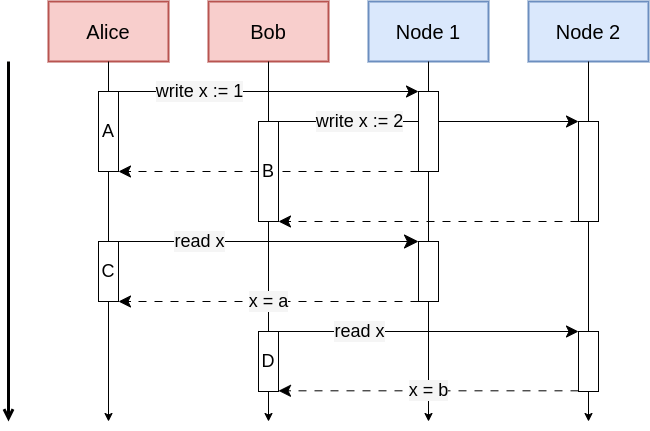
\includegraphics[scale=0.6]{images/Requests.png}
  \caption{A sequence of read/write requests. A consistency model constrains the possible values of $a$ and $b$.}
\end{figure}

A \emph{consistency model} is a constraint on the allowable system
responses to these sorts of request histories. In this example, a
model constrains the possible values of $a$ and $b$. The strongest
workable consistency model is linearizability
\cite{10.1145/78969.78972}, also known as atomic
consistency.\footnote{In the context of isolated database
transactions, the analogous condition is called strict serializability
or serializability with external order.} The intuition is that to an
outside observer, a linearizable system processes requests exactly as
if they were all being handled by one node, though not always in the
order they requests were received. For instance, two consecutive read
requests must return the same value, assuming no intermediate updates
take place between the two requests. When requests are seen to
overlap, such as the updates in our example, linearizability specifies
no order on their execution. In other words, the system must act as if
during some moment while processing the request, the update instantly
took effect, but this order doesn't have to be the order in which a
request was received if they are processed concurrently.

Applied to our example, linearizability allows either write request to
take effect before the other, but they both take effect before $a$ is
read by Client 1, so $a$ must be $1$ or $2$. $b$ must have the same
value as $a$, since it is read after reading $a$ and there are no
intermediate updates to $x$. Linearizability would be violated if $b
\neq a$ because an external observer could infer the clients are
operating on different, inconsistent copies of $x$.

Enforcing linearizability imposes appreciable performance overheads on
a system, as no agent can complete an update until the update has been
propagated to all other agents. Consequently, issues with a small
number of nodes can have a disproportionately disruptive impact on the
entire application. Unsurprisingly, real-world frameworks frequently
consider models weaker than linearizability.

One weaker model, but one still regarded as a form of ``strong''
consistency, is sequential consistency
\cite{1979LamportSequential}. Here, we weaken the requirement that
effects appear to happen in an order consistent with wall clock
time. The new requirement is that the effects \emph{from a single
client} must occur in their specified order (i.e. program order), but
requests from two different clients may appear to happen in any order,
even if they don't occur concurrently in real time. Sequential
consistency would require that both $a$ and $b$ can be either 1 or 2,
with no correlation. While a real-time observer can observe behavior
that looks inconsistent with real time, the basic intuition is that if
a history is always compatible with some temporal order that
\emph{could} have happened, this is all a programmer needs to reason
about the correctness of their applications. Linearizability implies
sequential consistency, and is sometimes called sequential consistency
plus (compatibility with) external order.

Both forms of strong consistency, atomic and sequential, are too
stringent to require from many applications, especially in an
unreliable communications environment, due to performance overheads.
This phenomenon is partly captured by the so-called CAP theorem, which
we now turn to.

\subsection{The consistency/availability tradeoff}

Real-world systems often fall short of behaving as a single perfectly
coherent system. The root of this phenomenon is that there exists a
deep and well-understood tradeoff between system coherence and system
performance. Enforcing consistency comes at the cost of additional
communications, and communications impose overheads, often ones that
can be unpredictable. The network may also fail to deliver messages or
rearrange their order. Such behavior presents obstacles to
consistency, particularly if the system should also exhibit good
performance.

Fox and Brewer \cite{1999foxbrewer} observed that there is a
fundamental tension between consistency, availability, and
partition-tolerance. This tradeoff was precisely stated and proved in
2002 by Gilbert and Lynch \cite{2002gilbertlynchCAP}. To summarize
this theorem, we start by defining these terms.

\paragraph{Consistency}

Consistency in Gilbert and Lynch is defined as atomic consistency
(linearizability). The CAP theorem can be also generalized to
sequential consistency. As discussed in \cite{2019wideningcap}, this
stronger theorem is essentially already proved by Birman and Friedman
\cite{10.5555/866855}.

\paragraph{Availability}

A CAP-available system is one that will definitely respond to every
client request at some point in the future. In particular, in the
event of a network partition that prevents messages from being
delivered, the system cannot indefinitely suspend processing requests
until the network recovers, as we do not assume partitions eventually
recover. In real applications we also care about the \emph{speed} with
which requests are handled, but the CAP theorem demonstrates there are
already obstacles to ensuring that every request is handled
\emph{eventually}.

\paragraph{Partition-tolerance}

A partition tolerant system continues to function, and ensure whatever
guarantees it is meant to provide, in the face of arbitrary partitions
in the network. Note that partitions may never recover, say if a
critical communications link is permanently severed.

\begin{theorem}[CAP Theorem]
In the presense of indefinite network partitions, a distributed system
cannot guarantee both atomic consistency and availability.
\end{theorem}

The proof is not complicated. Indeed, it is almost trivial. We give
only a sketch here, leaving the interested reader to consult Gilbert
and Lynch \cite{2002gilbertlynchCAP}. In the example above, suppose the two clients have
their requests served by two different system nodes, and suppose these
nodes cannot pass messages due to an indefinite network
partition. Linearizability requires that $a$ is $1$ or $2$ and $b =
a$.  Clearly $a$ cannot be $2$ if there is no communication between
the two clients. But clearly $b$ cannot be $1$ for the same reason.
To avoid violating the condition $b = a$ we could suppose the system
indefinitely delays responding to the read requests, but this violates
our requirement that system nodes eventually respond to
clients. Therefore, $P$ implies we cannot have both $C$ and $A$.

While the proof of the CAP theorem is rather trivial, its
interpretation is subtle and has been the subject of much discussion
in the years since \cite{2012CAP12Years}. It is sometimes assumed that
the CAP theorem claims that a distributed system can only offer two of
the properties C, A, and P. In fact, the theorem constrains, but does
not prohibit the existence of, applications that apply some relaxed
amount of all three features. The CAP theorem only rules out their
combination when all three are interpreted in a highly idealized
sense.

One way the the CAP theorem is idealized is that it defines
consistency as linearizability, a very strong condition. In practice
one often tolerates weaker levels of consistency. Also, network
partitions are often not as dramatic as an indefinite total
communications blackout. Real-world conditions in our context are
likely more chaotic, featuring many smaller disruptions and delays and
sometimes larger ones. Communications between different clients may be
affected differently, with nearby agents generally likely to have
better communication channels between them than agents that are far
apart. Finally, CAP-availability is a suprisingly weak condition. It
only requires that requests are handled eventually. In a truly highly
available system, we expect requests to be handled quickly almost
always. Altogether, the extremes of C, A, and P in the CAP theorem are
not reflective of most real-world applications.

The tension between consistency and availability is well-understood
\cite{10.1145/5505.5508}. It is a prototypical example of an even
broader tension in distributed systems: that between safey and
liveness properties \cite{2012perspectivesCAP}. These terms can be
understood as follows.

\paragraph{Safety}
Safety properties ensure that a system avoids doing something ``bad''
like violating a consistency invariant. Taken to the extreme, one way
to ensure safety is to do nothing. For instance, we could enforce
safety by never responding to read requests in order to avoid offering
information that is inconsistent with that of other nodes.

\paragraph{Liveness}
Liveness properties ensure that a system will eventually do something
``good'', like respond to a client. Taken to the extreme, one very
lively behavior would be to immediately respond to user requests,
without taking any steps to make sure this response is consistent with
that of other nodes.

Note that in our use cases, one can imagine that an unresponsive
system could indeed be considered ``unsafe.'' The distinction between
the two here is that safety constrains a system's allowable responses
to clients, if one is even given, while liveness requires giving
responses.

Because of the tension between them, building applications that
provide both of these features is challenging. The fundamental
principle is that if we want to increase how quickly a system can
respond to requests, eventually we must relax our constraints on what
the system is allowed to return. In light of this deep tradeoff and
the safety-critical nature of our use cases, the next section
enumerates three features of distributed applications we consider
particularly desirable in the contexts under consideration.
